\documentclass[11pt]{article}
\usepackage[margin=1.05in]{geometry}
\usepackage{amsmath,amssymb,amsthm}
\usepackage{booktabs}
\usepackage{graphicx}
\usepackage{xcolor}
\usepackage[colorlinks=true,linkcolor=blue!50!black,citecolor=blue!50!black,urlcolor=blue!50!black]{hyperref}
\usepackage{microtype}
\newtheorem*{rule*}{The rule}
\newcommand{\F}{\mathbb F}
\newcommand{\Z}{\mathbb Z}
\newcommand{\C}{\mathbb C}
\newcommand{\abar}{\bar\alpha}
\title{Reading the curve\\\large The stones, the rule and the cone, worked by hand on one curve of genus one}
\date{October 5, 2026}
\author{A reading note for the research record}
\begin{document}
\maketitle

\begin{abstract}
\noindent The note \emph{The cone over a curve} (\texttt{FUNCTION\_FIELD\_CONE.md}) showed that the light cone of the folds paper, carried over to a curve over a finite field, closes at the half-width $a=g\log q$, where $g$ is the genus. This note works the whole of that statement by hand on the smallest case, the curve $y^2=x^3+x^2+1$ over $\F_3$, in the language of the stones and the rule. Four ideas are needed: the point counts are the stones; a finite rule generates all of them; the Riemann Hypothesis for the curve says the rule's two numbers lie on a circle; and the proof of that comes from one floor up, from the maps of the curve to itself, not from the counts. Every number below can be checked with pencil and paper, and the machine checks are recorded where they were made.
\end{abstract}

\section{The curve and its stones}

Take the curve
\[
E:\quad y^2=f(x)=x^3+x^2+1\qquad\text{over }\F_3=\{0,1,2\}.
\]
It is smooth ($f$ and $f'=2x$ have no common root: $f(0)=1\neq0$), and a smooth cubic in this form has genus $g=1$. For each finite field $\F_{3^m}$ the stone $N_m$ is the number of solutions $(x,y)$ with $x,y\in\F_{3^m}$, plus one point at infinity. A value $x$ contributes two points if $f(x)$ is a nonzero square, one if $f(x)=0$, none if $f(x)$ is a nonsquare.

\paragraph{$N_1$ by hand.} Over $\F_3$ the only nonzero square is $1$.
\[
f(0)=1\ (\text{square: 2 points}),\qquad f(1)=3\equiv0\ (\text{1 point}),\qquad f(2)=8+4+1=13\equiv1\ (\text{2 points}).
\]
So $N_1=2+1+2+1=6$.

\paragraph{$N_2$ by hand.} $\F_9=\F_3[i]$ with $i^2=2$. Its nonzero squares are $1,2,i,2i$ (each is the square of something: $1=1^2$, $2=i^2$, $i=(1+2i)^2$, $2i=(1+i)^2$). The nine values of $x$:
\begin{center}
\begin{tabular}{lllc}
\toprule
$x$ & $f(x)$ & status & points \\
\midrule
$0$ & $1$ & square & 2\\
$1$ & $0$ & zero & 1\\
$2$ & $1$ & square & 2\\
$i$ & $2i$ & square & 2\\
$2i$ & $i$ & square & 2\\
$1+i$ & $2+i$ & nonsquare & 0\\
$1+2i$ & $2+2i$ & nonsquare & 0\\
$2+i$ & $0$ & zero & 1\\
$2+2i$ & $0$ & zero & 1\\
\bottomrule
\end{tabular}
\end{center}
Total $11$, plus infinity: $N_2=12$. (The rows for $2\pm i$ are the roots of $x^2+2x+2$, the factor of $f$ left after $x-1$; the whole factorization is $f=(x-1)(x^2+2x+2)$ over $\F_3$.)

\paragraph{Closed points.} The six $\F_3$-points are the closed points of degree $1$: $b_1=6$. The remaining six points over $\F_9$ fall into conjugate pairs under $i\mapsto2i$: the four points over $x=i,2i$ make two closed points of degree $2$, the two points over $x=2\pm i$ make one more. So $b_2=3$, and indeed $N_2=b_1+2b_2=6+6$. In the cone these are the prime powers: a closed point of degree $d$ sits at position $\log 3^d=d\log3$ on the prime line, with weight $d$, and enters the cone at half-width $a=\tfrac12 d\log 3$.

\section{The rule}

There is a map of the curve to itself, Frobenius, $\pi(x,y)=(x^3,y^3)$. Its fixed points over $\overline{\F}_3$ are exactly the $\F_3$-points, and the fixed points of $\pi^m$ are the $\F_{3^m}$-points. The theory (Hasse for genus one, Weil in general) says there are two numbers $\alpha,\abar$, the eigenvalues of Frobenius, with
\begin{equation}\label{eq:rule}
N_m=3^m+1-\alpha^m-\abar^m\qquad\text{for every }m\geq1,
\end{equation}
and $\alpha\abar=3$. Everything is therefore fixed by the single number $a_1=\alpha+\abar=3+1-N_1$. For our curve
\[
a_1=4-6=-2,\qquad \alpha,\abar\ \text{roots of}\ T^2+2T+3,\qquad \alpha=-1+i\sqrt2,\quad\abar=-1-i\sqrt2 .
\]
The zeta polynomial is $P(T)=1-a_1T+3T^2=1+2T+3T^2$, the same one \texttt{rh\_ff\_cone.py} produced from the counts.

\begin{rule*}
One number, $a_1=-2$, generates every stone there will ever be. The power sums come from Newton's identities, $\alpha^m+\abar^m=a_1(\alpha^{m-1}+\abar^{m-1})-3(\alpha^{m-2}+\abar^{m-2})$:
\[
\alpha^2+\abar^2=4-6=-2,\quad \alpha^3+\abar^3=-8+18=10,\quad \alpha^4+\abar^4=4-18=-14,
\]
hence the predictions
\[
N_2=9+1+2=12,\qquad N_3=27+1-10=18,\qquad N_4=81+1+14=96 .
\]
$N_2=12$ is the table above. $N_3=18$ and $N_4=96$ were counted by brute force in $\F_{27}$ and $\F_{81}$ (the engine of \texttt{rh\_ff\_cone.py}, 27 and 81 values of $x$): both agree.
\end{rule*}

This is the sense in which the genus is the size of the rule. A curve of genus $g$ has $2g$ eigenvalues; given the functional equation ($\alpha\mapsto q/\alpha$ permutes them) the first $g$ counts $N_1,\dots,N_g$ determine all of them, and without it the first $2g$ do. For $g=1$ the first count alone is the whole rule. After degree $2g$ the stones say nothing new; they are consequences.

\section{The Riemann Hypothesis for the curve}

The zeta function of $E$ is $\zeta_E(s)=Z(3^{-s})$ with $Z(T)=P(T)/((1-T)(1-3T))$, and its zeros are the $s$ with $3^{s}=\alpha$ or $\abar$. Their real part is $\log|\alpha|/\log3$. So
\[
\text{RH for }E\iff|\alpha|=|\abar|=\sqrt3\iff\text{all zeros have }\operatorname{Re}s=\tfrac12 .
\]
For our curve $|\alpha|^2=\alpha\abar=3$: true. Write $\alpha=\sqrt3\,e^{i\theta}$. Then $\cos\theta=-1/\sqrt3$, $\theta=\pm125.26^\circ$. The two zeros are two points on a circle, at angles $\pm\theta$; the imaginary parts of $s$ are periodic with period $2\pi/\log3$, which is why the circle replaces the line. The zero measure of the curve is $\nu_E=\delta_\theta+\delta_{-\theta}$.

\section{The cone, by hand}

The cone needs the Fourier coefficients of the zero measure, which the stones give directly:
\[
\hat\nu_E(m)=e^{im\theta}+e^{-im\theta}=\frac{\alpha^m+\abar^m}{3^{m/2}}=3^{m/2}+3^{-m/2}-\frac{N_m}{3^{m/2}} .
\]
\[
\hat\nu_E(0)=2,\qquad \hat\nu_E(1)=\frac{-2}{\sqrt3},\qquad \hat\nu_E(2)=\frac{-2}{3}.
\]
The Weil form at support $D$ is the quadratic form on sequences $h(-D),\dots,h(D)$,
\[
Q_D(h)=\sum_{j,k}h(j)h(k)\,\hat\nu_E(j-k)=\big|\hat h(\theta)\big|^2+\big|\hat h(-\theta)\big|^2,\qquad \hat h(\theta)=\sum_n h(n)e^{in\theta},
\]
and its matrix is the Toeplitz matrix $T_{2D+1}=[\hat\nu_E(j-k)]$. The form at support $D$ uses $\hat\nu_E(m)$ for $|m|\le2D$, that is, the stones $N_1,\dots,N_{2D}$: the closed points of degree $\le2D$, which are the ones inside the cone of half-width $a=D\log3$ (edge $\log n=2a$).

\paragraph{Support $D=0$, half-width $a=0$.} $T_1=[\,2\,]$. The floor is $2$. The cone knows there are two zeros and nothing about where they are: the identity phase of the atlas note on the potential set.

\paragraph{Support $D=1$, half-width $a=\log3=1.0986$.} The six degree-one stones entered at $a=\tfrac12\log3$; the three degree-two stones sit on the edge. The matrix is
\[
T_3=\begin{pmatrix}2&-\frac{2}{\sqrt3}&-\frac23\\[2pt]-\frac{2}{\sqrt3}&2&-\frac{2}{\sqrt3}\\[2pt]-\frac23&-\frac{2}{\sqrt3}&2\end{pmatrix}.
\]
Split into the even sequences $h=(p,s,p)$ and the odd ones $h=(p,0,-p)$.
\begin{itemize}
\item \emph{Odd sector.} $Q(p,0,-p)=2p^2\big(2-\hat\nu_E(2)\big)=2p^2\cdot\tfrac83$, so on unit vectors the odd floor is $\tfrac83=2.667$. Positive: the odd sector is still open.
\item \emph{Even sector.} In the orthonormal basis $(1,0,1)/\sqrt2$, $(0,1,0)$ the block is
\[
\begin{pmatrix}2+\hat\nu_E(2)&\sqrt2\,\hat\nu_E(1)\\ \sqrt2\,\hat\nu_E(1)&2\end{pmatrix}=\begin{pmatrix}\frac43&-\frac{2\sqrt2}{\sqrt3}\\[2pt]-\frac{2\sqrt2}{\sqrt3}&2\end{pmatrix},\qquad \det=\frac83-\frac83=0 .
\]
Its eigenvalues are $0$ and $\tfrac{10}3$. The floor of the whole form is $0$: \textbf{the cone has closed} at $a=g\log q=\log3$, exactly as the proposition says, and the machine run gave the same three eigenvalues $0,\ \tfrac83,\ \tfrac{10}3$ (\texttt{data/ff\_cone\_g1\_q3.json}).
\end{itemize}

\paragraph{The null vector returns the zeros.} Solve $T_3p=0$ with $p=(p_1,p_0,p_1)$. The middle row gives $p_0=-\hat\nu_E(1)\,p_1=\tfrac{2}{\sqrt3}p_1$; the first row then reads $2-\tfrac43-\tfrac23=0$, satisfied. So $p\propto(1,\tfrac{2}{\sqrt3},1)$, and the polynomial with these coefficients is
\[
w^2+\frac{2}{\sqrt3}w+1=0,\qquad w=-\frac{1}{\sqrt3}\pm i\sqrt{\tfrac23},\qquad |w|^2=\tfrac13+\tfrac23=1,\quad \cos(\arg w)=-\frac1{\sqrt3}.
\]
These are $e^{\pm i\theta}$: the two zeros, read off from nine stones at half-width $\log3$. In the number-field cone this is the step that never happens: there is no finite support at which the stones inside return the rule, because the rule there has infinitely many numbers in it.

\paragraph{One degree later.} At $D=2$ the odd sector closes too (its floor at $D=2$ is $0$ in the machine run), as the proposition predicts for $D=g+1$. From $D=1$ on, the rank of $T_{2D+1}$ stays at $2g=2$ and the potential set is the single measure $\nu_E$.

\section{Where the circle comes from: one floor up}

Nothing in Sections 1--4 explains why $|\alpha|=\sqrt3$. The counts cannot, on their own: \eqref{eq:rule} with any two numbers of product $3$ is a consistent-looking rule until one checks it against geometry. Hasse's proof (1933) uses one fact about maps of the curve to itself.

The maps $E\to E$ that respect the group law form a ring containing $\Z$ and $\pi$; every nonzero map $\phi$ has a \emph{degree}, the number of preimages of a general point, which is a nonnegative integer, and the degree is a quadratic form on the ring. The counts are degrees: $N_m=\deg(1-\pi^m)$, because a point is fixed by $\pi^m$ exactly when it is sent to the identity by $1-\pi^m$. Expanding the quadratic form on the elements $m-n\pi$ gives
\[
\deg(m-n\pi)=m^2-a_1\,mn+3\,n^2\geq0\qquad\text{for all integers }m,n .
\]
Check it on our curve: $\deg(1-\pi)=1+2+3=6=N_1$. A binary quadratic form that is nonnegative on all integer pairs (hence, by scaling, on all rational and real pairs) has discriminant $a_1^2-4\cdot3\le0$. So $|a_1|\le2\sqrt3$, the roots of $T^2-a_1T+3$ are complex conjugates, and $|\alpha|^2=\alpha\abar=3$. For our curve $a_1^2=4\le12$.

That is the whole proof, and notice where the positivity lives. It is not a property of the sequence $6,12,18,96,\dots$ It is the statement that a degree is a count of preimages and so cannot be negative, applied to maps that are not Frobenius powers at all ($2-\pi$, $3-2\pi$, and so on). The stones are the values of the form on the line $(1,-1),(1,-\pi^2),\dots$; the rule that forces the circle is the form's positivity on the whole lattice. The framework stands one floor above the counts and explains all of them at once.

For genus $g\geq2$ Weil (1948) replaced the endomorphism ring by the surface $X\times X$ and the degree by the intersection number of curves on it; the positivity is the Hodge index theorem (the Castelnuovo--Severi inequality), applied to the graph of Frobenius. The structure is the same: a quadratic form on a geometric object, nonnegative for a geometric reason, whose values on one line are the counts. The Weil form of the cone is this form in another basis, which is why its floor is nonnegative at every support and reaches zero exactly when the geometry has been fully used, at $D=g$.

\section{Back to the integers}

The dictionary is now concrete.
\begin{center}\small
\begin{tabular}{ll}
\toprule
curve $E/\F_3$ & the integers\\
\midrule
closed points of degree $d$, at $d\log3$ & prime powers $n$, at $\log n$\\
stones $N_1,N_2,\dots$, generated by $a_1$ & $\psi(x)$, generated by the zeros\\
rule: $2g=2$ numbers on a circle & rule: infinitely many zeros on a line\\
cone closes at $a=g\log q=\log3$ & cone never closes\\
floor exactly $0$ from $a=\log3$ on & floor positive at every $a$ computed, decaying\\
null vector at the horizon returns the zeros & no null vector at any finite $a$\\
positivity from the endomorphism ring (Hasse) & positivity for all $a$ \emph{is} RH (Weil's criterion)\\
\bottomrule
\end{tabular}
\end{center}
The statement ``the genus of $\zeta$ is infinite'' has a precise meaning in this picture: the rule has no finite size, the stones never run out, and the floor has no finite support at which to vanish. The comparison figure (\texttt{FUNCTION\_FIELD\_CONE.png}, reproduced below) shows the two behaviours side by side with the same coordinate $a$.

The thing nobody has is the right-hand column's last row with a reason in it: the object one floor above the integers whose positivity would be RH. Every serious attempt at RH by analogy is a search for that object: Deninger's foliated dynamical systems, Connes and Consani's arithmetic site, the field with one element. None has produced the surface. That is the honest frontier, and it is where the digging goes next.

\section*{Where to dig}
\begin{enumerate}\sloppy
\item Redo Section 4 for the genus-two curve $y^2=x^5+2x^3+2$ over $\F_3$ (\texttt{data/ff\_cone\_g2\_q3.json}): the cone should stay open at $D=1$ (floor $1$) and close at $D=2$. The $5\times5$ even block is still hand-sized.
\item Hasse's proof in full: Silverman, \emph{The Arithmetic of Elliptic Curves}, Chapter V, Theorem 1.1, with the reason that degree is a quadratic form.
\item Weil's for genus $g$, through the Hodge index theorem: Hartshorne, \emph{Algebraic Geometry}, Exercise V.1.10, and Milne's survey \emph{The Riemann hypothesis over finite fields from Weil to the present day} (2016), which also tells the story of the search for the integer analogue.
\end{enumerate}

\begin{center}
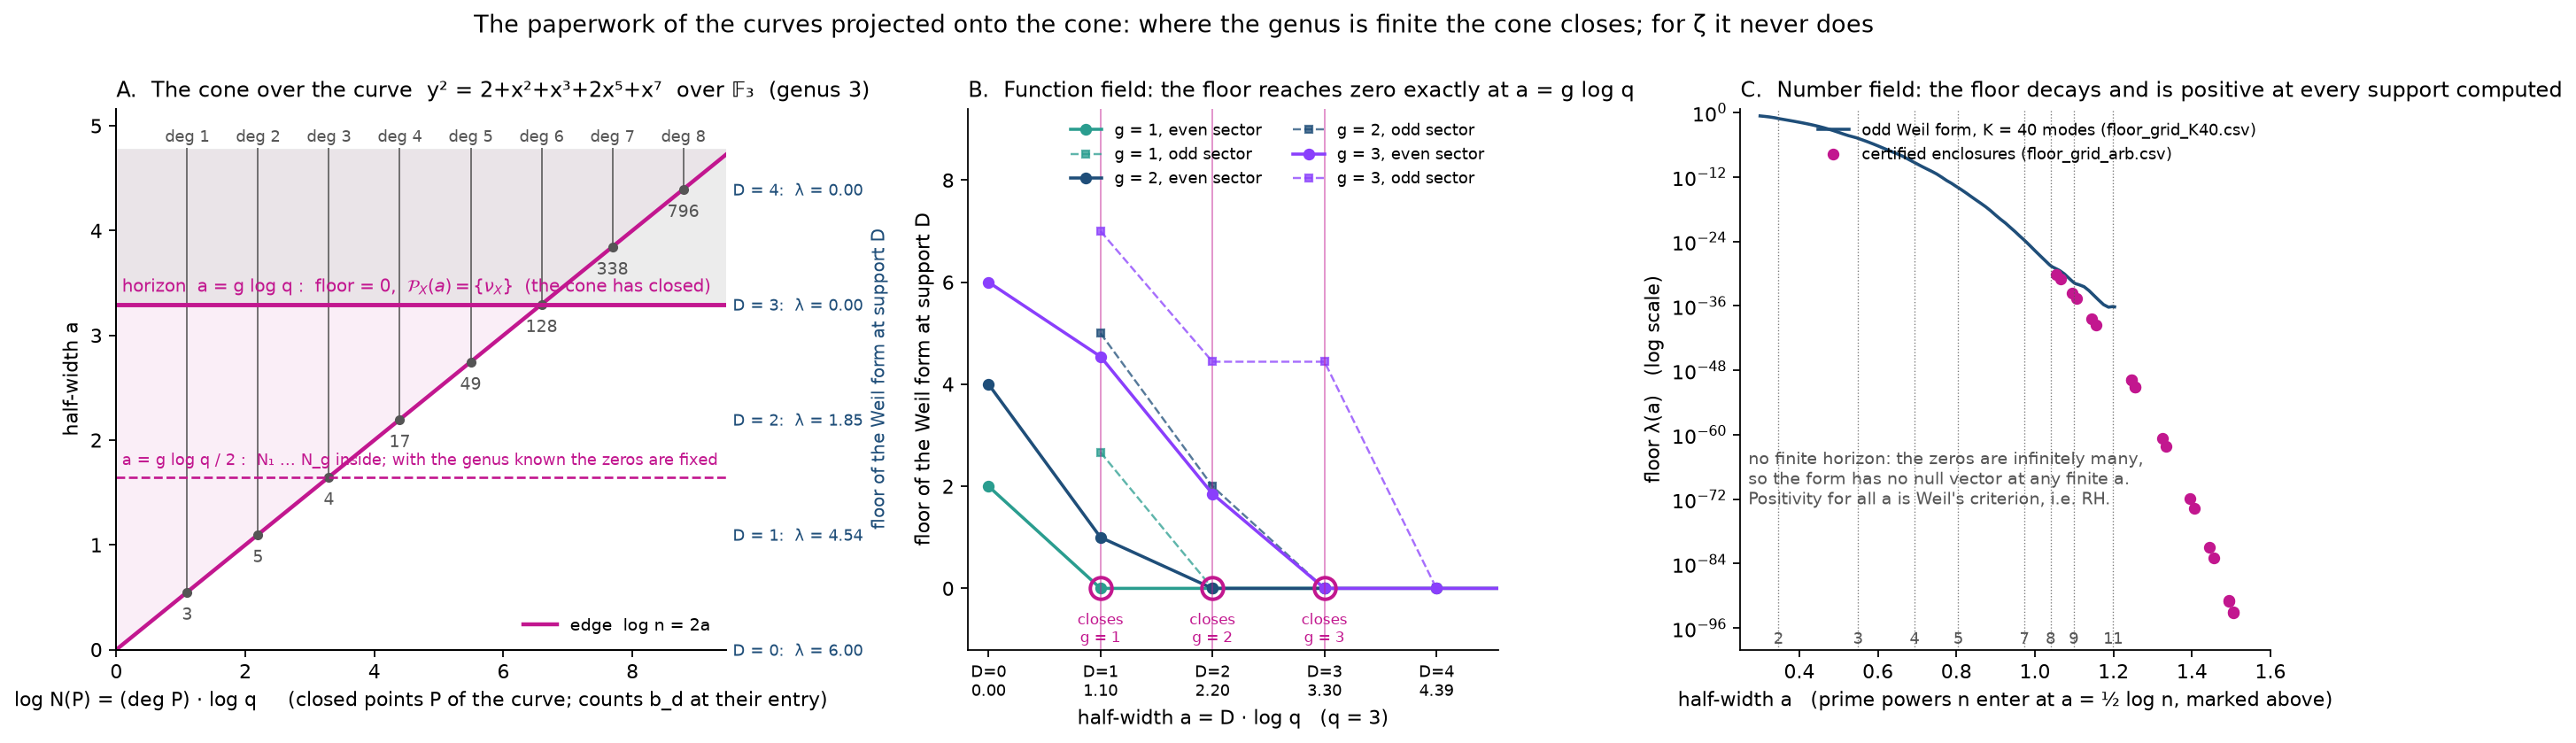
\includegraphics[width=\textwidth]{FUNCTION_FIELD_CONE.png}
\end{center}

\begin{thebibliography}{9}
\bibitem{hasse} H.~Hasse, Beweis des Analogons der Riemannschen Vermutung f\"ur die Artinschen und F.~K.~Schmidtschen Kongruenzzetafunktionen in gewissen elliptischen F\"allen, \emph{Nachr. Ges. Wiss. G\"ottingen} (1933), 253--262.
\bibitem{weil} A.~Weil, \emph{Sur les courbes alg\'ebriques et les vari\'et\'es qui s'en d\'eduisent}, Hermann, Paris, 1948.
\bibitem{silverman} J.~H.~Silverman, \emph{The Arithmetic of Elliptic Curves}, 2nd ed., Springer, 2009, Chapter V.
\bibitem{hartshorne} R.~Hartshorne, \emph{Algebraic Geometry}, Springer, 1977, Exercises V.1.9--1.10.
\bibitem{milne} J.~S.~Milne, The Riemann hypothesis over finite fields from Weil to the present day, in \emph{The Legacy of Bernhard Riemann after One Hundred and Fifty Years}, Int. Press, 2016.
\bibitem{deninger} C.~Deninger, Some analogies between number theory and dynamical systems on foliated spaces, \emph{Doc. Math.} Extra Vol. ICM I (1998), 163--186.
\bibitem{cc} A.~Connes and C.~Consani, Geometry of the arithmetic site, \emph{Adv. Math.} 291 (2016), 274--329.
\bibitem{ffcone} \emph{The cone over a curve}, \texttt{FUNCTION\_FIELD\_CONE.md}, this repository, 2026-10-05.
\bibitem{potential} \emph{The potential set of the light cone}, \texttt{atlas\_potential\_set.pdf}, this repository.
\end{thebibliography}
\end{document}
